\documentclass[sigconf,review,anonymous]{acmart}
\settopmatter{printacmref=false}
\renewcommand\footnotetextcopyrightpermission[1]{}
\acmConference[ISEC 2027]{Innovations in Software Engineering Conference}{2027}{Mumbai, India}
\acmYear{2027}
\acmDOI{}
\acmISBN{}
\setcopyright{none}

\usepackage{booktabs}
\usepackage{graphicx}
\usepackage{colortbl}
\usepackage{framed}
\raggedbottom
\definecolor{shadecolor}{RGB}{221,235,250}
\usepackage{microtype}
\setlength{\emergencystretch}{3em}

\newcommand\blfootnote[1]{%
  \begingroup
  \renewcommand\thefootnote{}\footnote{\raggedright #1}%
  \addtocounter{footnote}{-1}%
  \endgroup
}

\begin{document}

\title{CAST: Testing the Attribution Stability of AI-Generated-Code Detectors Under Controlled Source Transformations}

\author{Anonymous Author(s)}
\affiliation{\institution{Submission to ISEC 2027}\country{}}

\begin{abstract}
AI-generated-code detectors are evaluated almost exclusively on static snapshots, even though real code is routinely reformatted, renamed, and restructured after creation. A detector's verdict can feed an academic-integrity case, a hiring assessment, or an AI-disclosure policy, so a verdict that changes under a cosmetic edit is a real risk. We present CAST (Code Attribution Stability Testing), a controlled, distance-instrumented methodology that measures whether a detector's human-versus-AI attribution survives routine, non-adversarial transformations, with a canonicalization intervention to diagnose presentation-driven instability.

On 199 held-out Python and Java programs from the Droid corpus, reformatting with a standard tool (\texttt{black}/\texttt{google-java-format}) flips a reconstructed detector's (DroidDetect-Base) correct verdict on human-written code to ``AI'' 58.0\% of the time (29/50), against 2/105 on AI-authored code and 5.2\% (5/96) in a reverse perturbation (Fisher's exact $p{=}2.1{\times}10^{-12}$). The effect is concentrated in short programs (88\% in the shorter half of human programs, 28\% in the longer half) but persists at matched length, and it is not explained by edit size. The other two detectors show why a low instability rate is not evidence of robustness: LLMSniffer performs at or below a majority-class baseline on this corpus (67.0\% Python, 44.4\% Java), and DetectCodeGPT flips its decision on \emph{unchanged} input 30.0\% of the time, as often as under transformation. Canonicalization reduces DroidDetect-Base's residual movement 14.8--15.4$\times$, but the canonicalized input is often out-of-distribution for the detector, so it is not yet a mitigation. Static accuracy alone does not characterize detector reliability under routine code evolution.
\end{abstract}

\keywords{AI-generated code detection, robustness testing, metamorphic testing, software evolution, code authorship attribution}

\maketitle

\section{Introduction}

AI coding assistants now write a substantial share of the code developers review, edit, and ship. Detectors that attribute this code to a human or AI origin are typically evaluated the same way a classifier is: on a fixed test set, scored once, with accuracy as the verdict. That verdict is not academic. Detectors are already being proposed for academic-integrity enforcement in classrooms, screening in take-home hiring assessments, and compliance with project- or organization-level AI-disclosure policies. A false accusation in any of these settings has a real person on the other end of it.

The standard evaluation protocol quietly assumes the code being judged stays put. It does not. An IDE reformats a file on save, a refactor renames a variable, a reviewer rewrites a loop; none of it changes what the program does, yet any of it can change what a detector says about who wrote it. A detector whose verdict flips under a cosmetic edit is not measuring origin; it is measuring the snapshot.

This is a routine, non-adversarial threat, and it is distinct from the adversarial setting the closest prior work targets. Robustness studies for AI-code detectors vary how the code is generated in the first place~\cite{hidinginplainsight}, not how it changes afterward. Detector papers that do report a robustness number typically report it for one perturbation at most, with no stratified account of which kinds of edits matter and why. Work explicitly adversarial to detectors trains a classifier against an attacker's renaming strategy~\cite{codegptsensorplus} or evaluates under deliberately adversarial generation and rewriting scenarios~\cite{droid}. Separate lines of work show that renaming alone can defeat a code watermark~\cite{codewatermark}, and that metamorphic testing of code models more broadly treats identifier renaming as a standard, non-adversarial transformation~\cite{metamorphicslr}. None of this literature measures whether an already-trained, unmodified AI-code detector's verdict survives a non-adversarial edit that a developer or a tool would make anyway, or reports which specific kinds of edits matter and why.

This paper's objective is to make attribution stability an explicit, measurable property of an AI-code detector, not an afterthought to accuracy, and to build the smallest instrument that can measure it. We introduce \textbf{CAST} (Code Attribution Stability Testing): given a program of known origin, CAST applies a validated transformation, measures the resulting change at the text, token, and AST level, and records how the detector's score and decision move. Where movement is large, CAST adds a second, targeted step: canonicalizing both sides of the pair to test whether the instability is a presentation artifact or something deeper.

Applied to three detectors over 199 held-out Python and Java programs~\cite{droid}, this approach exposes what a single accuracy number cannot. One detector shows a large, class-specific, false-accusing instability under formatting, strongly modulated by program length, that canonicalization only partially and ambiguously attenuates. For the other two, the low or high instability we measure is uninterpretable, because of degenerate baseline accuracy and re-scoring noise, respectively.

This paper makes two contributions.
\begin{itemize}
\item \textbf{CAST}, a controlled, distance-instrumented diagnostic methodology for evaluating the attribution stability of already-trained AI-code detectors under routine, non-adversarial edits. The canonicalization intervention and the identity-transformation noise-floor control guard against two confounds that affected two of our three detectors: apparent stability that reflects degenerate baseline accuracy (LLMSniffer), and apparent instability that cannot be separated from re-scoring noise (DetectCodeGPT).
\item An empirical result: a reconstructed detector (DroidDetect-Base, 86.4\% four-class accuracy on the test corpus, consistent with its dev-split check) shows a large, class-specific, directionally asymmetric instability under reformatting: correct human-code verdicts flip to ``AI'' far more often than the reverse (Fisher's exact $p{<}10^{-11}$), concentrated in short programs but present at matched length. This is consistent with the detector treating tidy formatting as a proxy for AI authorship.
\end{itemize}

The remainder of the paper is organized as follows. Section~2 defines CAST and the canonicalization intervention. Section~3 describes the dataset, transformations, detectors, and research questions. Section~4 reports results. Section~5 discusses their implications. Section~6 lists threats to validity. Section~7 positions CAST against related work. Section~8 outlines future plans, and Section~9 concludes. An Artifact Availability Statement follows the conclusion.

\begin{figure*}[t]
\centering
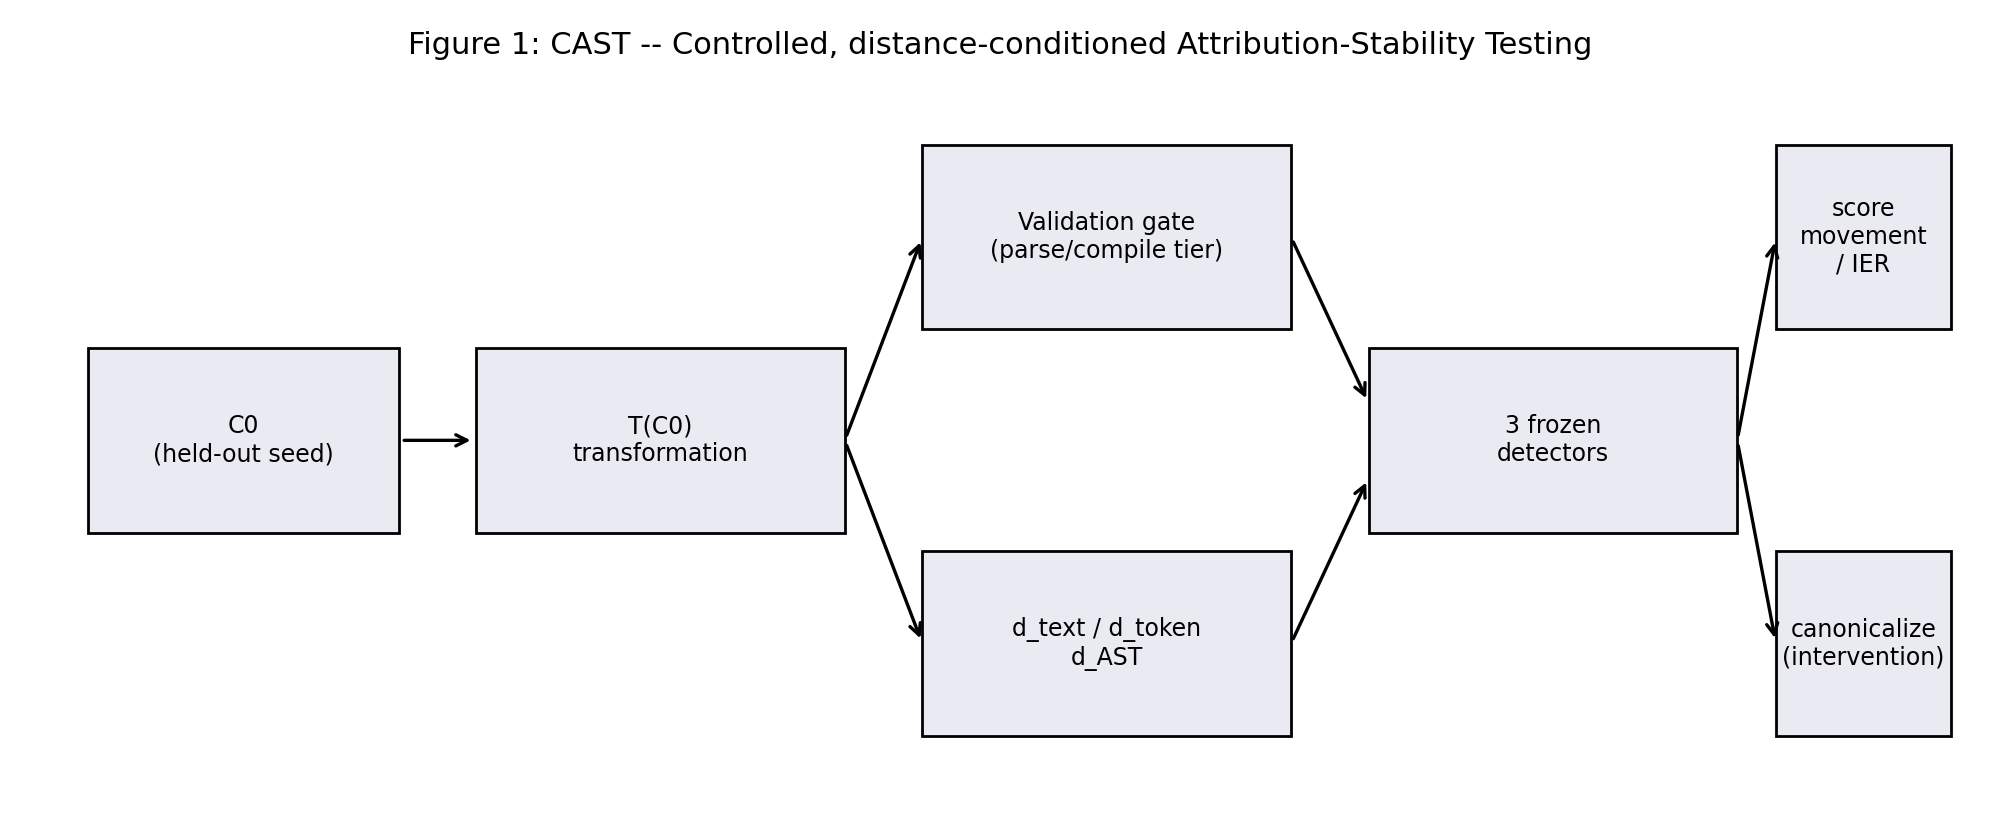
\includegraphics[width=0.92\textwidth]{figures/figure1_cast_methodology.png}
\caption{The CAST framework: main pipeline (top), canonicalization intervention (middle), and identity-transformation noise-floor control (bottom).}
\label{fig:cast}
\end{figure*}

\section{CAST}

This section introduces CAST (Code Attribution Stability Testing), the diagnostic framework this paper uses to measure how AI-generated-code detectors respond to routine, non-adversarial source transformations, summarized in Figure~\ref{fig:cast}. Section~\ref{sec:attribution-stability} defines attribution stability and distinguishes it from adversarial robustness; Section~\ref{sec:methodology} details the five-step measurement pipeline and the Induced Error Rate; and Sections~\ref{sec:noise-floor} and~\ref{sec:canon} introduce two controls, an identity-transformation noise floor and a canonicalization intervention, used to separate genuine instability from measurement noise and presentation-driven confounds, respectively.

\subsection{Attribution stability}
\label{sec:attribution-stability}

\emph{Attribution stability} is the degree to which a detector's output for a program is preserved under routine, non-adversarial edits, distinct from adversarial robustness, which studies a worst-case attacker searching for an evasive rewrite. CAST's transformations are fixed, deterministic operators applied uniformly across the corpus, not an adversarial search against any particular detector. CAST treats score movement and decision-flip rate as first-class observations, rather than reducing the evaluation to a single post-transformation accuracy number.

\subsection{Methodology}
\label{sec:methodology}

For a detector $D$, a transformation $T$, and a program $C_0$ of known provenance, CAST proceeds in five steps, illustrated in Figure~\ref{fig:cast}.
\begin{enumerate}
\item Apply $T$ to obtain $T(C_0)$.
\item Validate that $T(C_0)$ is well-formed at or above $C_0$'s own syntactic-validity tier. Non-applicable and invalid outcomes are recorded, not discarded, so that applicability itself is a reportable quantity.
\item Measure $d_\text{text}$ (character-level edit distance), $d_\text{token}$ (edit distance over the language's own lexical token stream: Python's \texttt{tokenize} output including \texttt{INDENT}/\texttt{DEDENT}, or Java tree-sitter leaves), and $d_\text{AST}$ (AST node-count change), so that the magnitude of an edit can later be related to the magnitude of a detector's response.
\item Score $D(C_0)$ and $D(T(C_0))$.
\item Aggregate, per detector, language, and transformation family, the mean and median score movement $\Delta_D = D(T(C_0)) - D(C_0)$, the decision-flip rate, and the \textbf{Induced Error Rate}, defined as:
\end{enumerate}
\begin{equation}
\text{IER} = \frac{\#\{\text{baseline-correct programs whose decision flips after } T\}}{\#\{\text{baseline-correct programs}\}}
\end{equation}

IER is conditioned on the detector having been correct on $C_0$. A flip on a program the detector already misclassified would otherwise conflate ordinary detector error with transformation-induced instability, understating the difference between a detector that is simply inaccurate and one that is accurate but unstable. Detectors also expose incompatible score semantics across implementations: a calibrated probability, an uncalibrated sigmoid output, or an unnormalized statistic with no fixed range. CAST therefore does not compare raw $|\Delta_D|$ across detectors. IER, a bounded proportion with a consistent interpretation regardless of the underlying score scale, is the primary cross-detector metric; raw score movement is interpreted only within a given detector's own distribution, never compared across detectors directly.

\subsection{Identity-transformation noise floor}
\label{sec:noise-floor}

Some detectors are not deterministic at inference time: a statistic computed from a sampled or randomly perturbed process can, in principle, return a different verdict on literally unchanged input simply because the random seed differed. Before attributing any instability to the transformation itself, CAST re-scores $C_0$ against itself with a fresh random seed and no transformation applied, and reports the resulting decision-flip rate and mean $|\Delta|$ as a noise floor. A detector's transformation-induced IER is only interpretable relative to this floor: an IER within the range of the noise floor cannot be distinguished from measurement noise, no matter how elevated it looks in isolation. Deterministic detectors (no sampling at inference) have a zero noise floor by construction, and this control is skipped for them.

\subsection{Canonicalization intervention}
\label{sec:canon}

When a transformation family produces large score movement, CAST additionally scores $F(C_0)$ and $F(T(C_0))$ for a deterministic canonicalizer $F$ that removes a specific, named category of variation: in this study, whitespace, blank lines, comments, and quote style, implemented by re-tokenizing the program and rejoining its semantic tokens. A pair for which $F(C_0) = F(T(C_0))$ collapses to $\Delta = 0$ by construction. This subset is reported separately from the residual pairs for which a genuine difference remains after canonicalization, so that the diagnostic result is not an artifact of the trivially-resolved cases inflating an average. A substantial reduction in the residual subset's score movement constitutes intervention evidence that the removed category of variation contributes to the observed instability. It does not constitute proof of a specific internal mechanism, and, as this paper's own results show, it can be confounded by the canonicalized input itself becoming out-of-distribution for the detector under test, a limitation of this particular canonicalizer, not of the diagnostic logic in general.

\section{Study Design}

This section describes how CAST is instantiated for this study. Section~3.1 introduces the dataset of 199 held-out programs; Section~3.2 defines the three confirmatory transformation families; Section~3.3 explains how the validity of each transformed program is checked; Section~3.4 describes the three detectors evaluated and how each was obtained; and Section~3.5 states the three research questions the evaluation is built around.

\subsection{Dataset}

This evaluation uses DroidCollection's~\cite{droid} held-out test split. We requested 100 Python and 100 Java programs, stratified by provenance label and, for the two machine labels, by generator family, using a fixed random seed and excluding the pilot programs used to develop the pipeline. One Java draw collided with a pilot program and was dropped by the disjointness guard, leaving 199 programs (100 Python, 99 Java): 66 \texttt{HUMAN\_GENERATED} (33 Python, 33 Java), 67 \texttt{MACHINE\_GENERATED} (33, 34), and 66 \texttt{MACHINE\_REFINED} (34, 32). The 66 human-written programs come mostly from library-style code fragments (The Vault function, class, and inline subsets: 44), with 11 competitive-programming solutions (TACO), 10 StarCoder files, and 1 AtCoder solution. \texttt{MACHINE\_REFINED} denotes human-written code that has been modified or extended by a language model, a collaborative category distinct from either pure human authorship or pure machine generation.

\subsection{Transformations}

Three families are treated as confirmatory: formatting (\texttt{black} for Python, \texttt{google-java-format} for Java), lexical renaming of one identifier, and control-flow rewriting (one canonical loop-form rewrite). Of the 597 attempted (program, family) pairs, 229 were not applicable (for example, no loop to rewrite), 3 failed validation, and 365 succeeded; these give an applicability rate of 0.616 (368/597) and a success rate among applicable attempts of 0.992 (365/368). A fourth stage attempted two deeper transformation families, local structural extraction and semantics-preserving rewriting, at two intensities each; this stage is reported as a feasibility finding, not a confirmatory one, because of the corpus-composition limitation described there.

\subsection{Validation}

Python validity is checked via \texttt{compile()}. Java is tiered, given the corpus's substantial share of function- and class-level fragments rather than complete compilation units: \texttt{STANDALONE\_VALID} $>$ \texttt{WRAPPER\_VALID} (compiles only inside a synthetic harness, used as a validation instrument and never itself scored) $>$ \texttt{STRUCTURAL\_ONLY} $>$ \texttt{PARSE\_INVALID}.

\subsection{Detectors}

Of five targeted detectors, two had a released checkpoint runnable as-is; a third, DroidDetect-Base, required reconstructing its architecture from the checkpoint alone, since no modeling code was published for it.

\textbf{LLMSniffer}~\cite{llmsniffer} (GraphCodeBERT~\cite{graphcodebert} with a supervised-contrastive head) reaches 90.0\% sanity-check accuracy on GPTSniffer's own Java test subset~\cite{gptsniffer}, but only 67.0\% (Python) and 44.4\% (Java) on this study's 199-program baseline, at or below a majority-class baseline of 67.0\%/66.7\% respectively. This gap between its published in-domain accuracy and its out-of-domain accuracy on Droid is itself informative: a detector's reported accuracy figure does not transfer automatically to a new corpus, and this paper's methodological point, that a low IER needs a baseline-accuracy check, would not have been visible without measuring it directly on the same corpus used for the stability evaluation.

\textbf{DroidDetect-Base} (ModernBERT-base~\cite{modernbert} with a projection layer and a four-class classification head) ships a public checkpoint with no accompanying modeling code. We reconstructed its architecture from the checkpoint's own parameter names and shapes. The only choices made on a disjoint dev-split subset of 24 programs (six per Droid label) were the pooling mode and the label order; the reconstruction reaches 87.5\% exact four-class accuracy there (Wilson 95\% CI [69.0, 95.7]). On the 199-program test corpus, the same reconstruction reaches 86.4\% exact four-class accuracy (172/199, CI [81.0, 90.5]), consistent with the dev figure, and 98.5\% (196/199) on the binary human-versus-AI collapse used for all IER results. These are different metrics and should not be compared with each other: on AI-class programs, four-class accuracy is 106/133 (79.7\%) but binary accuracy is 130/133 (97.7\%), because most four-class errors confuse \texttt{MACHINE\_GENERATED} with \texttt{MACHINE\_REFINED}. The reconstruction has not been compared against the original authors' own numbers and the dev check is small, so because the central finding rests on this one detector, we treat it as the main threat to validity.

\textbf{DetectCodeGPT}~\cite{detectcodegpt} is a zero-shot statistic from the DetectGPT~\cite{detectgpt}/NPR~\cite{detectllm} family, computed by perturbing the input with masked-span fill-in and comparing log-likelihoods under CodeLlama-7B~\cite{codellama} and CodeT5p-770M~\cite{codet5plus}. A pre-registered convergence study established that no perturbation count $K{<}50$ satisfies a predeclared convergence criterion against the $K{=}50$ reference, so $K{=}50$ perturbations are used throughout. Its decision threshold, calibrated on an independent 40-sample set, reaches only 60.0\% accuracy, near chance, so its raw score movement is treated as the primary evidence in this study, and its threshold-derived binary decisions as secondary, lower-confidence evidence.

\textbf{GPTSniffer}~\cite{gptsniffer} and \textbf{CodeGPTSensor/+}~\cite{codegptsensor} could not be integrated into this study, as neither released a pretrained checkpoint at the time of writing. We deliberately did not train replacements from scratch, since doing so would introduce confounds (training-data composition, hyperparameter choices, our own implementation bugs) distinct from evaluating a detector as its own authors published and validated it.

\subsection{Research Questions}

This evaluation is structured around three research questions.
\begin{itemize}
\item \textbf{RQ1:} How stable are detector scores and decisions under formatting, lexical renaming, and control-flow rewriting?
\item \textbf{RQ2:} Do detectors exhibit similar or detector-specific stability profiles under identical transformations, and are apparent differences genuine or artifacts of baseline accuracy or measurement noise?
\item \textbf{RQ3:} Does canonical normalization attenuate transformation-associated instability, and does this differ across detectors?
\end{itemize}

\section{Results}

This section reports the results, organized by research question. Section~4.1 answers RQ1 and RQ2, comparing the three detectors' Induced Error Rates across transformation families and languages and testing the central human-to-AI versus AI-to-human asymmetry; Section~4.2 answers RQ3 by applying the canonicalization intervention; and Section~4.3 reports, as a feasibility finding rather than a confirmatory one, how far the corpus supports deeper transformation families.

\subsection{RQ1/RQ2: detector-specific, transformation-specific profiles}

Table~\ref{tab:ier} reports IER with baseline-correct denominators, for all three detectors across all three confirmatory transformation families and both languages. DroidDetect-Base's formatting IER exceeds its lexical-rename and control-flow IER in both languages, collapsing to at or near 0\% under both of the other transformations in Python. Wilson~\cite{wilson1927} 95\% confidence intervals for formatting do not overlap those of the other two families in Python; Java's smaller post-collapse denominators give wider, overlapping intervals, so the effect is directionally consistent in Java but less sharply statistically separated there than in Python.

\begin{table}[t]
\centering
\footnotesize
\setlength{\tabcolsep}{3pt}
\caption{Induced Error Rate by detector, language, and transformation family ($n$ = baseline-correct; $\dagger$ = secondary evidence, weak calibration). Green: IER $\le$5\%.}
\label{tab:ier}
\begin{tabular}{@{}llccc@{}}
\toprule
Detector & Language & Family & IER (n) & 95\% CI \\
\midrule
DroidDetect-Base & Python & \textbf{formatting} & \textbf{26.1\% (24/92)} & [18.2,35.9] \\
DroidDetect-Base & Java & \textbf{formatting} & \textbf{11.1\% (7/63)} & [5.5,21.2] \\
DroidDetect-Base & Python & lexical rename & \cellcolor{green!20}0.0\% (0/80) & [0.0,4.6] \\
DroidDetect-Base & Java & lexical rename & \cellcolor{green!20}1.2\% (1/82) & [0.2,6.6] \\
DroidDetect-Base & Python & control flow & \cellcolor{green!20}0.0\% (0/26) & [0.0,12.9] \\
DroidDetect-Base & Java & control flow & 6.2\% (1/16) & [1.1,28.3] \\
LLMSniffer & Java & formatting & 8.3\% (2/24) & [2.3,25.8] \\
LLMSniffer & Python & formatting & 6.5\% (4/62) & [2.5,15.4] \\
LLMSniffer & Python & lexical rename & \cellcolor{green!20}1.9\% (1/52) & [0.3,10.1] \\
LLMSniffer & Java & lexical rename & \cellcolor{green!20}0.0\% (0/35) & [0.0,9.9] \\
LLMSniffer & Python & control flow & \cellcolor{green!20}0.0\% (0/15) & [0.0,20.4] \\
LLMSniffer & Java & control flow & \cellcolor{green!20}0.0\% (0/4) & [0.0,49.0] \\
DetectCodeGPT$^\dagger$ & Python & control flow & 50.0\% (7/14) & [26.8,73.2] \\
DetectCodeGPT$^\dagger$ & Python & lexical rename & 30.2\% (13/43) & [18.6,45.1] \\
DetectCodeGPT$^\dagger$ & Python & formatting & 25.0\% (12/48) & [14.9,38.8] \\
DetectCodeGPT$^\dagger$ & Java & formatting & 16.7\% (6/36) & [7.9,31.9] \\
DetectCodeGPT$^\dagger$ & Java & lexical rename & 16.7\% (8/48) & [8.7,29.6] \\
DetectCodeGPT$^\dagger$ & Java & control flow & 18.2\% (2/11) & [5.1,47.7] \\
\bottomrule
\end{tabular}
\end{table}

Table~\ref{tab:byclass} breaks the formatting result down further, by the program's \emph{true} origin class rather than pooling across all AI-authored code: DroidDetect-Base's formatting IER is 58.0\% (29/50) on genuinely human-written code, but only 0.0\% (0/58) on machine-generated code and 4.3\% (2/47) on machine-refined code, a pattern that holds consistently when Python and Java are examined separately (Python: 66.7\%/0.0\%/6.5\%; Java: 41.2\%/0.0\%/0.0\%). This class-specific asymmetry is not a no-op artifact of the transformation simply doing nothing to already-tidy AI code: only 5--6\% of AI-class formatting transformations leave the code byte-identical to its input.

\begin{table}[t]
\centering
\footnotesize
\setlength{\tabcolsep}{3pt}
\caption{DroidDetect-Base formatting IER by true origin class. Green: IER $\le$5\%.}
\label{tab:byclass}
\begin{tabular}{@{}lccc@{}}
\toprule
True class & $n$ (baseline-correct) & IER & 95\% CI \\
\midrule
\textbf{HUMAN\_GENERATED} & 50 & \textbf{58.0\% (29/50)} & [44.2,70.6] \\
MACHINE\_GENERATED & 58 & \cellcolor{green!20}0.0\% (0/58) & [0.0,6.2] \\
MACHINE\_REFINED & 47 & \cellcolor{green!20}4.3\% (2/47) & [1.2,14.3] \\
\bottomrule
\end{tabular}
\end{table}

To test this asymmetry more directly, we ran a reverse experiment: messifying AI-class code (introducing trailing whitespace, extra blank lines, and inconsistent quoting and spacing: a deterministic, semantics-preserving, validity-checked transformation) on the 106 of 133 AI-class programs whose exact four-class label DroidDetect-Base predicted at baseline, of which 96 remained after excluding 10 whose messified output failed validation, and measuring the reverse, AI-to-human flip rate. This induces a flip in only 5/96 cases (5.2\%, 95\% CI [2.2, 11.6]; Python 6.5\%, Java 4.0\%), far below the 58.0\% human-to-AI rate. Conditioning on the exact four-class label is stricter than the binary decision used for the formatting IER; 24 AI-class programs that were correctly called AI but assigned the wrong AI subclass were not scored under messify. The comparison is also not intensity-matched: messify's mean length-normalized edit size ($d_\text{text}/\text{len} = 0.064$) is smaller than formatting's on human code ($\approx$0.14), so the gap confirms a real, directional asymmetry rather than measuring a matched effect size.

Program length strongly modulates the human-to-AI flips. Flipped human programs are much shorter than unflipped ones (mean 650 vs.\ 3531 characters), and the flip rate is 22/25 (88\%) in the shorter half of human programs against 7/25 (28\%) in the longer half (Spearman $\rho{=}{-}0.64$ between log length and flip). In a logistic regression on the 50 human formatting pairs, log length is the only significant predictor (odds ratio 0.12 per standard deviation, $p{<}0.001$); normalized edit size and language are not ($p{=}0.73$ and $0.54$). The class asymmetry does not depend on length: among programs of at most 1,000 characters, 25/30 human-written programs flip against 2/64 AI-class programs (Fisher's exact $p{=}1.1{\times}10^{-15}$), and the contrasts at 1,500 and 2,500 characters are similar (27/33 vs.\ 2/87; 28/37 vs.\ 2/102). The headline 58.0\% is thus a corpus-level average over a strongly length-dependent effect, with short human programs most exposed.

The difference between transformation families is not simply an edit-size effect either. On human-written code, lexical renaming and control-flow rewriting produce normalized edits of at most 0.26 of program length (medians 0.033 and 0.061) and flip in 0/75 pairs, whereas formatting pairs of comparable size (normalized edit at most 0.26) flip in 25/45. Within formatting, the flip rate does not rise with edit size (3/6, 12/18, 7/16, and 7/10 for normalized edits of below 0.05, 0.05--0.10, 0.10--0.20, and at least 0.20). This does not rule out that larger renaming or rewriting edits would flip more; we did not test them.

Score movement correlates only weakly with edit size: $|\Delta|$ has a Spearman correlation of $\rho{=}0.22$ with $d_\text{text}$ for DroidDetect-Base and $\rho{=}0.30$ for LLMSniffer. The correlations with $d_\text{AST}$ ($\rho{=}{-}0.20$ and $0.03$) carry little information, because formatting leaves the AST node count unchanged by construction, so $d_\text{AST}$ is zero for almost all formatting pairs.

Of the 29 flipped human programs, the four-class output lands mostly on \texttt{MACHINE\_REFINED} (17/29) rather than \texttt{MACHINE\_GENERATED} (11/29), with one on \texttt{MACHINE\_GENERATED\_\allowbreak ADVERSARIAL}. Droid defines \texttt{MACHINE\_REFINED} as human-written code modified by an \emph{LLM}; a deterministic formatter is not an LLM, so we count these verdicts as false accusations.

LLMSniffer's low IER (below 8.3\% throughout; full per-family results in Table~\ref{tab:ier}) is not, by itself, evidence of robustness: its own baseline accuracy on this corpus is 67.0\% in Python (exactly its majority-class baseline, i.e., indistinguishable from a constant predictor) and 44.4\% in Java (\emph{below} its 66.7\% majority-class baseline, i.e., anti-correlated with the true label more often than not). A detector with no signal, or negative signal, on a corpus will trivially show a low decision-flip rate simply because it is not tracking the input's content in the first place.

DetectCodeGPT's IER is elevated broadly across all three families (16.7--50.0\%, secondary evidence given its weak calibration), peaking under control-flow rather than formatting, a diffuse pattern with no clear family-specific localization. An identity-transformation control (Section~2.3), re-scoring 40 frozen dev-split samples with an unchanged input but a freshly seeded perturbation set, found a comparably sized 30.0\% decision-flip rate and a mean $|\Delta|$ of 0.925, larger than the transformation-induced movement reported in Table~\ref{tab:canon}. DetectCodeGPT's elevated IER therefore cannot currently be distinguished from its own re-scoring noise.

The 58.0\% (29/50) human-to-AI rate and the 5.2\% (5/96) AI-to-human rate come from independent samples (different programs), so we test the asymmetry with Fisher's exact test rather than a paired test: the difference is extreme (odds ratio 25.1, $p{=}2.1{\times}10^{-12}$), confirming the asymmetry is not attributable to chance even setting aside the non-overlapping confidence intervals already reported.

\par\addvspace{4pt}\noindent\colorbox{shadecolor}{\parbox{\dimexpr\columnwidth-2\fboxsep\relax}{%
\textbf{Answer to RQ1/RQ2:} DroidDetect-Base's formatting instability is real, class-specific, and directionally asymmetric (58.0\% vs.\ 5.2\%, Fisher's exact $p{<}10^{-11}$, not intensity-matched). It is concentrated in short programs but holds at matched length, and edit size alone does not explain it. The other two detectors do not yield interpretable stability estimates on this corpus: LLMSniffer's low IER reflects accuracy at or below chance, and DetectCodeGPT's high IER (16.7--50.0\%) is comparable to its 30.0\% flip rate on unchanged input. A low IER is therefore not evidence of robustness without a baseline-accuracy check and a noise-floor control.
}}\par\addvspace{4pt}


\subsection{RQ3: canonicalization intervention}

The canonicalization diagnostic was applied to all 158 formatting pairs (94 Python, 64 Java). Canonicalizing both sides collapsed 108/158 (68.4\%) to byte-identical input ($\Delta{=}0$ by construction); the remaining 50/158 retained a genuine residual difference and were rescored. Table~\ref{tab:canon} reports both the full-set and residual-only figures, so that the diagnostic's real contribution is isolated from the trivially-resolved majority of pairs.

\begin{table*}[t]
\centering
\caption{Mean $|\Delta|$ before/after canonicalization (raw scores, comparable only within a detector). Green: reduction $\ge$3$\times$.}
\label{tab:canon}
\begin{tabular*}{\textwidth}{@{}@{\extracolsep{\fill}}llcccc@{}}
\toprule
Detector & Lang. & \multicolumn{2}{c}{Full set} & \multicolumn{2}{c}{Residual-only} \\
 & & before & after (red.) & before & after (red.) \\
\midrule
LLMSniffer & Py (94/32) & 0.027 & \cellcolor{green!20}0.003 (8.6$\times$) & 0.032 & \cellcolor{green!20}0.009 (3.5$\times$) \\
LLMSniffer & Java (64/18) & 0.025 & \cellcolor{green!20}0.002 (16.7$\times$) & 0.020 & \cellcolor{green!20}0.005 (3.7$\times$) \\
\textbf{DroidDetect-Base} & Py (94/32) & 0.315 & \cellcolor{green!20}0.009 (\textbf{34.9$\times$}) & 0.394 & \cellcolor{green!20}0.027 (\textbf{14.8$\times$}) \\
\textbf{DroidDetect-Base} & Java (64/18) & 0.161 & \cellcolor{green!20}0.003 (\textbf{63.3$\times$}) & 0.139 & \cellcolor{green!20}0.009 (\textbf{15.4$\times$}) \\
DetectCodeGPT & Py (94/32) & 0.687 & 0.280 (2.5$\times$) & 0.843 & 0.824 (1.0$\times$) \\
DetectCodeGPT & Java (64/18) & 0.645 & 0.244 (2.6$\times$) & 0.566 & 0.866 (\textbf{0.7$\times$, increase}) \\
\bottomrule
\end{tabular*}
\end{table*}

On the residual-only subset, DroidDetect-Base's mean score movement still falls 14.8--15.4$\times$ after canonicalization. This reduction, however, is complicated by an out-of-distribution effect that this paper measured directly rather than assumed away: on the 100 canonicalized residual scores, DroidDetect-Base's mean probability assigned to the \emph{true} class drops to 0.223, with 66\% of these scores below 0.05, against 98.5\% binary baseline accuracy on unmodified input. Canonicalized input is therefore often confidently \emph{misclassified} by this detector, meaning the large apparent reduction in score movement may partly reflect the model failing in a different, more uniform way on out-of-distribution input, rather than genuinely recognizing the code as origin-preserved once presentation differences are removed. DetectCodeGPT shows no comparable reduction on the residual subset (Python 1.0$\times$, i.e.\ essentially unchanged; Java 0.7$\times$, i.e.\ an \emph{increase} in movement, from a mean $|\Delta|$ of 0.566 to 0.866), and its canonicalized scores skew toward the AI decision (68\% above its calibrated threshold, versus 50--54\% on unmodified baseline input), a further sign of distributional shift under canonicalization, not evidence against instability. LLMSniffer shows a smaller, genuinely real reduction on an already low baseline, with no comparable saturation signature. Pooled over languages, the residual-only reduction factors are 3.6$\times$, 14.9$\times$, and 0.9$\times$ for LLMSniffer, DroidDetect-Base, and DetectCodeGPT; we report residual-only factors deliberately, since the 68\% of pairs that collapse trivially would otherwise inflate the full-set numbers.




\par\addvspace{4pt}\noindent\colorbox{shadecolor}{\parbox{\dimexpr\columnwidth-2\fboxsep\relax}{%
\textbf{Answer to RQ3:} This particular canonicalizer cannot cleanly answer RQ3 for DroidDetect-Base: canonicalized input is itself frequently misclassified, so the large residual-movement reduction is confounded with a saturation/out-of-distribution effect rather than being clean evidence of resolved instability. A layout-preserving normalizer, which keeps canonicalized input closer to the detector's training distribution, is needed before this question can be settled with confidence. DetectCodeGPT's movement is unreduced by canonicalization, and on Java, larger afterward, evidence against, not for, a presentation-driven explanation of its instability.
}}\par\addvspace{4pt}

\subsection{Corpus feasibility for deeper transformations}

Local structural extraction and semantics-preserving rewriting were additionally attempted at two intensities each, as a feasibility probe for deeper transformation families beyond the three confirmatory ones. Of 796 attempted (language, family, intensity) combinations, only 37 (4.65\%) were applicable at all, of which 35 validated successfully; only 4 of those 35 received true differential-execution verification (i.e., actually running the program before and after the transformation and comparing outputs), with the remaining 31 degrading to structural-only validation for lack of an unambiguous, stdin-free entry point to execute. This outcome directly reflects Droid's composition: a substantial share of its rows are function- or class-level code fragments rather than complete, independently executable programs, which sharply bounds how densely this evaluation style currently extends to deeper, more realistic transformations. The resulting per-detector cells ($n{=}1$--$12$) are illustrative only and support no confirmatory claim; we report them for transparency about what was attempted and why it did not scale, not as evidence for or against any detector's stability.

\section{Discussion}

Static accuracy does not characterize post-transformation reliability, but this study's results show something further and less obvious: neither does a low Induced Error Rate, by itself, characterize genuine stability. LLMSniffer's near-majority-class (or, in Java, below-majority-class) accuracy on this corpus makes its low IER a likely artifact of a degenerate, near-constant, or even anti-correlated predictor rather than a sign of real robustness. DetectCodeGPT's IER is not yet separable from its own re-scoring noise, measured directly via the identity-transformation control rather than assumed to be negligible. Only DroidDetect-Base's instability survives both of these checks: it is a detector with high baseline accuracy (98.5\% binary, 86.4\% four-class) whose formatting sensitivity is reproducible under deterministic inference, class-specific, and directionally asymmetric under a genuinely different, reverse intervention (58.0\% vs.\ 5.2\%; Section~4.1).

The length-matched asymmetry in Section~4.1, more than the raw edit-distance comparison, is what best supports the interpretation that the detector has learned tidy formatting as a proxy signal for AI authorship, rather than genuinely modeling origin. CAST does not identify the underlying mechanism directly; that would require inspecting the detector's internal representations or its training data, which is outside this paper's scope. But the observable behavior, a large, reproducible, and one-sided sensitivity to a purely cosmetic, deterministic transformation, is consistent with a detector that has, whether intentionally or not, absorbed code style as a shortcut for origin during training. That short human programs are most exposed is consistent with a detector that has less content-level evidence to override a formatting cue, but we did not test this.

This finding motivates reporting stability under transformation as a standard companion to accuracy for any detector intended for real-world use, and suggests canonicalization as a lightweight diagnostic worth running before deploying a detector, even though this paper's own results show that the specific token-rejoining canonicalizer used here is not yet a validated mitigation; its own out-of-distribution effect means a practical fix likely requires a layout-preserving normalizer that keeps canonicalized code closer to a detector's training distribution, rather than one that strips presentation information as aggressively as this study's diagnostic canonicalizer does.

A verdict that cannot survive a random seed, or cannot survive a formatter being run on otherwise-unmodified code, is unfit for the single-verdict, high-stakes use this paper's motivation describes. The practical implication for anyone deploying or relying on an AI-code detector is not simply ``use a more accurate detector,'' but ``demand evidence of attribution stability, checked against both a baseline-accuracy floor and a re-scoring-noise floor, before trusting any individual verdict.''

For an instructor, hiring team, or compliance reviewer evaluating whether to adopt a specific detector, this paper's results translate into a concrete pre-deployment checklist: (1) measure the detector's own accuracy on a sample of your target corpus, not just its published number, since Section~3.4 shows these can diverge sharply; (2) run an identity-transformation control (Section~2.3) to establish a re-scoring noise floor before trusting any reported instability rate; (3) run the detector on the same file before and after an IDE's default formatter, and treat any flip on human-authored code as a false-accusation risk specifically, not a generic error rate, since this paper's asymmetry result suggests false accusations of human authors, not missed detections of AI authors, are where a formatter-sensitive detector fails; and (4) do not adopt a detector for a single-verdict, high-stakes decision until it has been checked against all three of the confounds this paper identifies (baseline accuracy, noise floor, and formatting sensitivity).

\section{Threats to Validity}

\textbf{External validity.} This evaluation covers two languages, one corpus, and three detectors; two additional targeted detectors could not be integrated because no checkpoint was released for either. Only one of the three detectors yields an interpretable stability estimate on this corpus, so the empirical finding is a case study of one detector, not a comparison across detectors. Training replacements for the missing detectors would have introduced confounds of their own. The transformation operators used represent common tooling edits (an automatic formatter, a single rename, a single loop rewrite), not a sampled distribution of real developer edit histories, which may differ in composition and intensity.

\textbf{Construct validity.} LLMSniffer's baseline accuracy on this corpus (67.0\% Python, at its own majority-class baseline; 44.4\% Java, below its majority-class baseline) means its low IER cannot be read as robustness evidence under any interpretation. Program length modulates the human-to-AI flips strongly (Section~4.1); we control for it by length-matched comparison and regression, but the short human programs in this corpus are mostly library-style fragments, so the estimate may not transfer to complete programs. The messify reverse check is not intensity-matched with formatting, so it establishes directionality, not a comparable effect size. DetectCodeGPT's weak calibration limits its threshold-derived binary results to secondary status throughout, and its reported IER and $|\Delta|$ are upper bounds that include a comparably sized identity-control noise floor rather than a clean estimate of transformation-induced instability alone. Detector scores have incompatible scales across implementations (Section~2.2), and $d_\text{text}$, $d_\text{token}$, and $d_\text{AST}$ correlate only weakly with $|\Delta|$ even for the detector with the clearest instability signal, meaning distance is a useful but incomplete proxy for how much a detector's output should be expected to move.

\textbf{Internal validity.} DroidDetect-Base's architecture was reconstructed from its checkpoint in the absence of any public modeling code, and this reconstruction has not been compared numerically against the original authors' own reported results. It reaches 87.5\% four-class accuracy on a 24-program dev subset and 86.4\% on the 199-program test corpus, but the dev check is small, and the paper's central finding rests on this one detector. The identity-control noise floor uses 40 dev-split programs rather than the test corpus, and a shared-seed variant that would reduce DetectCodeGPT's measurement noise was not run. DroidDetect-Base's IER throughout this paper uses the human-versus-AI collapse of its underlying four-class output, not raw four-class flips; of the 365 successful transformed pairs examined for this collapse, 23 were intra-AI churn (between \texttt{MACHINE\_GENERATED} and \texttt{MACHINE\_REFINED}); of those, 16 were among baseline-correct pairs and were excluded from IER on the grounds that they do not change the human-versus-AI verdict. The canonicalizer used in Section~4.2 normalizes several distinct presentation properties simultaneously (whitespace, blank lines, comments, and quote style), so a positive result from it supports a claim about that combined category of variation, not about which specific property within it is responsible; canonicalized-input accuracy, now measured and reported directly rather than assumed, shows a real out-of-distribution effect for DroidDetect-Base that the observed movement reduction does not fully control for.

\textbf{Corpus-composition validity.} Droid's fragment-heavy composition limits the deeper transformation families examined in Section~4.3 to 4.65\% applicability, and limits differential-execution verification specifically to 4 of 35 successful instances; the corresponding per-detector cells are illustrative only, not confirmatory, and should not be read as evidence for or against stability under those deeper transformations.

\textbf{Conclusion validity.} Some cells in this study's tables have small baseline-correct denominators, as low as $n{=}4$; Wilson 95\% confidence intervals are reported throughout specifically for this reason, rather than relying on point estimates alone. Cohen's $d_z$~\cite{cohen1988}, reported in the accompanying artifact, is treated only as supplementary, directional-consistency evidence, never as a headline statistic, since it can overstate practically small movements once standardized by variance.

\section{Related Work}

Measuring prediction change under fixed, semantics-preserving transformations is an established methodology for code models generally, and CAST does not claim novelty for that general idea. Rabin et al.~\cite{rabin} show that neural program models fail to generalize under a range of semantic-preserving program transformations. ReCode~\cite{recode} benchmarks code-generation robustness under more than 30 similarly-styled operators applied to prompts and completions. Both establish, for code models broadly, exactly the kind of result CAST is built to produce for AI-code detectors specifically: that a model's output can change substantially under an edit that does not change what the program does. CAST's contribution is applying this established style of test to a different task and a different failure mode: attribution false-accusation, framed explicitly as a metamorphic relation~\cite{metamorphicslr}, rather than degraded generation quality; and to a task (human-versus-AI attribution) where the practical stakes of an unstable verdict are qualitatively different from a worse code completion.

Table~\ref{tab:novelty} is a coarse positioning against the closest prior work, not a claim that CAST is better on any dimension; we regard the contribution as an application of an established testing style to AI-code detectors plus an empirical finding, not a new testing paradigm. It compares along four dimensions: whether the work edits code post-generation at all, whether that edit is routine rather than adversarial, whether the work targets already-trained AI-code detectors specifically (as opposed to code models in general or human-authorship attribution), and whether it compares multiple detectors under identical edits. Detector papers themselves~\cite{gptsniffer,llmsniffer,detectcodegpt,codegptsensor} report accuracy, occasionally under one perturbation, but do not stratify by transformation family or instrument edit distance. CodeGPTSensor+~\cite{codegptsensorplus} and Droid~\cite{droid} share this paper's underlying observation that renaming and refactoring can obscure AI origin, but address it through adversarial training or explicitly adversarial attack scenarios, not by measuring an already-trained, unmodified detector's stability under a non-adversarial edit. Pordanesh et al.~\cite{hidinginplainsight} vary the training set and prompting conditions used to \emph{generate} the code under test, not the source code itself after generation. RoPGen~\cite{ropgen} applies style transformation \emph{during training} to harden a \emph{human}-authorship attributor against stylistic evasion; CAST instead applies controlled transformation \emph{at evaluation time}, against \emph{already-trained}, unmodified AI-versus-human detectors, which is a materially different setting: RoPGen asks whether a detector can be trained to resist style manipulation, while CAST asks whether existing, deployed detectors already fail under style changes nobody intended as an attack. Feature-based work identifying whitespace as a particularly discriminative signal for AI-code detection~\cite{whitespaces} helps motivate, after the fact, why this paper's finding that formatting sensitivity is so strongly presentation-driven for DroidDetect-Base is plausible rather than surprising.

\begin{table*}[t]
\centering
\caption{Coarse positioning against the closest prior work.}
\label{tab:novelty}
\begin{tabular*}{\textwidth}{@{}@{\extracolsep{\fill}}lcccc@{}}
\toprule
Work & Post-gen. edit & Routine, non-adv. & AI-code detector & Cross-det. \\
\midrule
Detector papers~\cite{gptsniffer,llmsniffer,detectcodegpt,codegptsensor} & partial & partial & \checkmark & -- \\
CodeGPTSensor+~\cite{codegptsensorplus}, Droid~\cite{droid} & \checkmark & -- (adversarial) & \checkmark & partial \\
Pordanesh et al.~\cite{hidinginplainsight} & -- & -- & \checkmark & \checkmark \\
RoPGen~\cite{ropgen} & \checkmark & \checkmark & -- (human authorship) & -- \\
Code-model robustness~\cite{rabin,recode,codewatermark,metamorphicslr} & \checkmark & \checkmark & -- & partial \\
\textbf{CAST (this work)} & \checkmark & \checkmark & \checkmark & \checkmark \\
\bottomrule
\end{tabular*}
\end{table*}

\section{Future Plans}

This evaluation will be extended in four directions, prioritized by how directly they close the gaps identified in Section~6.

First, and highest priority, strengthening the validation of DroidDetect-Base's reconstruction: validating it on a larger dev sample (several hundred programs), comparing its outputs numerically against the original authors' own reported results where those become available, and contacting the original authors directly. Since this paper's central finding depends on this one reconstructed detector, this is the single highest-value next step.

Second, running an intensity-matched version of the reverse messify experiment (Section~4.1), calibrating the messiness transformation's normalized edit size to match formatting's on human code as closely as possible, so that the 58.0\%/5.2\% asymmetry can be reported as a properly matched effect-size comparison rather than only a directional one; alongside this, extending the identity-transformation noise-floor control from the current 40-sample dev-split subset to the full 199-program test set, and rescuing DetectCodeGPT's signal, where possible, with shared perturbation seeds across $C_0$ and $T(C_0)$ to reduce its measurement noise directly rather than only reporting it; and adding at least one further working detector, for example a model fine-tuned on Droid's training split, so that the empirical finding no longer rests on a single detector.

Third, replacing or supplementing the token-rejoining canonicalizer used in Section~4.2 with a layout-preserving normalizer, one that corrects specific presentation properties (indentation width, quote style, blank-line count) individually while leaving the code's overall structure closer to what the detector was trained on, together with a component-level ablation (whitespace-only, comments-only, quote-style-only) to determine which specific presentation property drives DroidDetect-Base's instability, rather than only the combined category this study currently reports.

Fourth, extending the corpus itself: a collection of complete, independently executable programs with test suites and chained, multi-step transformations mined from real commit histories, to scale beyond the 4.65\% applicability of the deeper transformation families documented in Section~4.3, and to substitute a sampled distribution of real developer edits for the tooling-driven transformations used throughout this study. Longer term, this points toward a detector explicitly trained against CAST's transformation families, to test directly whether attribution stability can be achieved by construction, rather than only diagnosed after the fact as this paper does.

\section{Conclusion}

This paper presented CAST, a controlled, distance-instrumented methodology for testing the attribution stability of AI-generated-code detectors under routine, non-adversarial source transformations. Applied to three detectors over 199 held-out Python and Java programs, its clearest finding is that a reconstructed detector (86.4\% four-class and 98.5\% binary accuracy on the test corpus) flips correct verdicts on human-written code to ``AI'' 58.0\% of the time after routine reformatting, against 2/105 on AI-authored code and 5.2\% under a reverse perturbation. The effect is concentrated in short programs but persists at matched length, consistent with the detector treating tidy formatting as a proxy for AI authorship. The other two detectors do not yield interpretable stability estimates on this corpus: LLMSniffer's low IER reflects accuracy at or below chance, and DetectCodeGPT's instability is indistinguishable from its re-scoring noise. Static accuracy alone does not characterize a detector's reliability under routine code evolution, and neither does a low instability rate by itself.

\section*{Artifact Availability Statement}

An anonymized artifact accompanies this submission at \url{https://anonymous.4open.science/r/cast-isec2027-artifact-461E}, mirroring a GitHub repository scrubbed of author-identifying information for double-blind review. An archival copy of the code and data (version 1.1.0) is deposited on Zenodo, \url{https://doi.org/10.5281/zenodo.22972809}. The artifact directly supports every quantitative claim in this paper and consists of:

\begin{itemize}
\item \textbf{Scripts} implementing the full CAST pipeline: manifest and transformation construction (formatting, lexical renaming, control-flow rewriting, and the deeper structural/semantic-rewrite families of Section~4.3), the three detector wrappers (LLMSniffer, the reconstructed DroidDetect-Base, and DetectCodeGPT), the canonicalization intervention, the identity-transformation noise-floor control (Section~2.3), the reverse ``messify'' experiment (Section~4.1), the human-vs-AI four-class-to-binary reclassification used throughout, the Fisher's exact test and the length and edit-size confound analysis reported in Section~4.1, and the table/figure generation scripts that produce every number and plot reported in the paper directly from frozen result files, with no manual editing step in between.
\item \textbf{Frozen result artifacts}: JSONL score files and derived CSV tables for every experiment phase, including the full per-family breakdowns for all three detectors (Table~\ref{tab:ier} reports these in full; no result is hidden or held back), the per-origin-class breakdown underlying Table~\ref{tab:byclass}, the canonicalization before/after scores underlying Table~\ref{tab:canon}, and the identity-control and messify-experiment raw outputs.
\item \textbf{Documentation}: a README describing how to regenerate every table and figure from the frozen artifacts (no GPU or model download required for this step), a Docker build file and a pinned Python dependency list for turnkey environment setup, pre-registration and results write-ups for each experimental phase, and an environment snapshot recording the software versions and hardware used to produce the original results.
\end{itemize}

Reproducing the tables and figures from the frozen artifacts requires no manual environment setup: a provided Docker build file builds a container with pinned dependencies and regenerates every table and figure in this paper (\texttt{docker build}, then \texttt{docker run}), which we verified end-to-end while preparing this artifact; a pinned dependency list is also provided for reproducing the same tables/figures in a local Python environment without Docker. Reproducing the underlying detector scores from raw code, rather than from the frozen artifacts, requires the three detectors' own dependencies (documented in the artifact) and, for DetectCodeGPT, GPU access, since it depends on CodeLlama-7B and CodeT5p-770M; this heavier path is intentionally kept outside the Docker image. Detector model checkpoints and cached Hugging Face model weights are not redistributed in the artifact, as they are large, third-party, and already publicly hosted at the citations given in Section~3.4; the artifact's environment snapshot records their exact versions and provenance. We intend to submit this artifact for evaluation and are targeting the \emph{Available}, \emph{Functional}, and \emph{Reusable} badges.

\begin{thebibliography}{99}

\bibitem{droid} D.~Orel, I.~Paul, I.~Gurevych, P.~Nakov, ``Droid: A Resource Suite for AI-Generated Code Detection,'' \emph{Proceedings of the 2025 Conference on Empirical Methods in Natural Language Processing (EMNLP)}, 2025.

\bibitem{llmsniffer} M.~L.~Dihan, A.~Muhtasim, ``LLMSniffer: Detecting LLM-Generated Code via GraphCodeBERT and Supervised Contrastive Learning,'' arXiv:2604.16058, 2026.

\bibitem{gptsniffer} P.~T.~Nguyen, J.~Di Rocco, C.~Di Sipio, R.~Rubei, D.~Di Ruscio, M.~Di Penta, ``GPTSniffer: A CodeBERT-based classifier to detect source code written by ChatGPT,'' \emph{Journal of Systems and Software}, 2024.

\bibitem{detectcodegpt} Y.~Shi, H.~Zhang, C.~Wan, X.~Gu, ``Between Lines of Code: Unraveling the Distinct Patterns of Machine and Human Programmers,'' \emph{Proceedings of the 47th International Conference on Software Engineering (ICSE)}, 2025.

\bibitem{codegptsensor} X.~Xu, C.~Ni, X.~Guo, S.~Liu, X.~Wang, K.~Liu, X.~Yang, ``Distinguishing LLM-generated from Human-written Code by Contrastive Learning,'' \emph{ACM Transactions on Software Engineering and Methodology}, vol.~34, no.~91, 2025.

\bibitem{codegptsensorplus} X.~Yin, X.~Li, C.~Ni, X.~Xu, X.~Yang, ``Detecting LLM-generated Code with Subtle Modification by Adversarial Training,'' arXiv:2507.13123, 2025.

\bibitem{codewatermark} T.~Suresh, S.~Ugare, G.~Singh, S.~Misailovic, ``Is the Watermarking of LLM-Generated Code Robust?'' arXiv:2403.17983, 2024.

\bibitem{metamorphicslr} A.~Asgari, M.~de Koning, P.~Derakhshanfar, A.~Panichella, ``Metamorphic Testing of Deep Code Models: A Systematic Literature Review,'' arXiv:2507.22610, 2025.

\bibitem{rabin} M.~R.~I.~Rabin, N.~D.~Q.~Bui, K.~Wang, Y.~Yu, L.~Jiang, M.~A.~Alipour, ``On the Generalizability of Neural Program Models with respect to Semantic-Preserving Program Transformations,'' \emph{Journal of Systems and Software}, 2021.

\bibitem{recode} S.~Wang, Z.~Li, H.~Qian, C.~Yang, Z.~Wang, M.~Shang, V.~Kumar, S.~Tan, B.~Ray, P.~Bhatia, R.~Nallapati, M.~K.~Ramanathan, D.~Roth, B.~Xiang, ``ReCode: Robustness Evaluation of Code Generation Models,'' \emph{Proceedings of the 61st Annual Meeting of the Association for Computational Linguistics (ACL)}, 2023.

\bibitem{hidinginplainsight} S.~Pordanesh, S.~Bukhari, B.~Tan, L.~De Carli, ``Hiding in Plain Sight: On the Robustness of AI-Generated Code Detection,'' \emph{Proceedings of the 22nd Conference on Detection of Intrusions and Malware, and Vulnerability Assessment (DIMVA)}, 2025.

\bibitem{ropgen} Z.~Li, G.~Q.~Chen, C.~Chen, Y.~Zou, S.~Xu, ``RoPGen: Towards Robust Code Authorship Attribution via Automatic Coding Style Transformation,'' \emph{Proceedings of the 44th International Conference on Software Engineering (ICSE)}, 2022.

\bibitem{whitespaces} S.~M.~H.~Nirob, S.~Ehsan, M.~Rahman, S.~Haque, ``Whitespaces Don't Lie: Feature-Driven and Embedding-Based Approaches for Detecting Machine-Generated Code,'' arXiv:2601.19264, 2026.

\bibitem{detectgpt} E.~Mitchell, Y.~Lee, A.~Khazatsky, C.~D.~Manning, C.~Finn, ``DetectGPT: Zero-Shot Machine-Generated Text Detection using Probability Curvature,'' arXiv:2301.11305, 2023.

\bibitem{detectllm} J.~Su, T.~Y.~Zhuo, D.~Wang, P.~Nakov, ``DetectLLM: Leveraging Log Rank Information for Zero-Shot Detection of Machine-Generated Text,'' \emph{Findings of the Association for Computational Linguistics: EMNLP 2023}, 2023.

\bibitem{codellama} B.~Rozi\`ere, J.~Gehring, F.~Gloeckle, et al., ``Code Llama: Open Foundation Models for Code,'' arXiv:2308.12950, 2023.

\bibitem{codet5plus} Y.~Wang, H.~Le, A.~D.~Gotmare, N.~D.~Q.~Bui, J.~Li, S.~C.~H.~Hoi, ``CodeT5+: Open Code Large Language Models for Code Understanding and Generation,'' arXiv:2305.07922, 2023.

\bibitem{modernbert} B.~Warner, A.~Chaffin, B.~Clavi\'e, et al., ``Smarter, Better, Faster, Longer: A Modern Bidirectional Encoder for Fast, Memory Efficient, and Long Context Finetuning and Inference,'' arXiv:2412.13663, 2024.

\bibitem{graphcodebert} D.~Guo, S.~Ren, S.~Lu, et al., ``GraphCodeBERT: Pre-training Code Representations with Data Flow,'' arXiv:2009.08366, 2020.

\bibitem{wilson1927} E.~B.~Wilson, ``Probable Inference, the Law of Succession, and Statistical Inference,'' \emph{Journal of the American Statistical Association}, vol.~22, no.~158, pp.~209--212, 1927.

\bibitem{cohen1988} J.~Cohen, \emph{Statistical Power Analysis for the Behavioral Sciences}, 2nd ed. Lawrence Erlbaum Associates, 1988.

\end{thebibliography}

\end{document}
